


\section{Markov para la ritmica}
\subsection{Informalmente}
El modelo est\'a basado en cadenas de markov. Al procesar un tema, lo que se hace es primero es estimar la \emph{metrical 
grid}, y luego elegir un nivel de la \emph{metrical grid} para dividir el tema.
Una vez elegido el nivel, dado que todos los beats del mismo nivel deben de estar equidistantes, se calcula el 
tiempo efectivo en el tema que hay entre dos beats consecutivos del nivel deseado (o mayor o igual), llamemoslo $t$.
Es importante notar que estas partes en las que se divide el tema no necesariamente corresponden con un comp\'as.

\begin{figure}[h]
\begin{center}
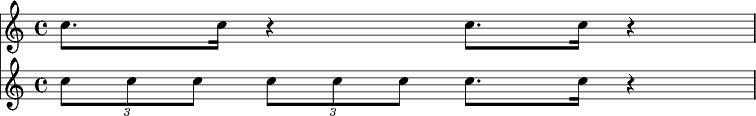
\includegraphics[width=12cm]{rythm_markov/images/reggae.png}
\label{fig:reggae}
\end{center}
\end{figure}

En el ejemplo, la \emph{metrical grid} es la de un comp\'as de $\frac{4}{4}$, y se dividir\'ia en dos partes, los dos renglones.

Dado que lo importante en la r\'itmica son los puntos de ataque, se podr\'ia preprocesar la entrada eliminando los silencios, y  
extendiendo la duraci\'on de la golpe anterior al silencio para que abarque tambi\'en el silencio.

De esta forma se generan potencialmente tantos estados como n\'umeros naturales haya menores a $t$ (y se los etiqueta con este n\'umero).
Luego para colocar las aristas entre los nodos se recorre la lista de golpes, y desde el nodo actual, llam\'emoslo
$n$, (que inicialmente es el nodo etiquetado como 0) se agrega una transicion al nodo $n+k$ modulo $t$,
donde $k$ es la duraci\'on del golpe en cuesti\'on.

Una vez terminado esto, puede ser que no sea posible hacer una random walk porque haya un estado (el correspondiente al \'ultimo golpe del tema, si 
este esta por la mitad de una parte) 
que no tiene transiciones salientes, de esta forma se agrega una transicion desde este estado hasta el estado mas cercano
que tenga transiciones salientes.

\begin{figure}[h]
\begin{center}
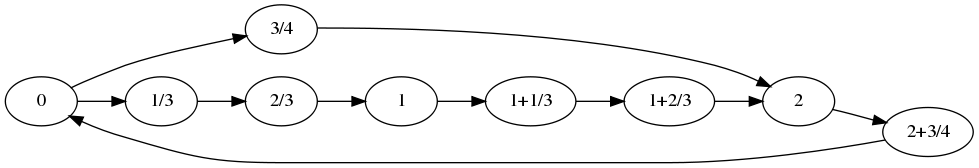
\includegraphics[width=12cm]{rythm_markov/images/grafo_sin_etiquetas.png}
\label{fig:grafo_sin_etiquetas}
\end{center}
\end{figure}

Sin embargo, al analizar este grafo, se puede ver que puede que sea conveniente analizar los silencios para aumentar el grado de entrada de los nodos
(permitiendo asi generar una mayor cantidad de variaciones). En el siguiente grafo se incluye los silencios, y para distinguirlos de los golpes que 
suenan, se agregan dos etiquetas a las transiciones \emph{R} para el silencio (Rest), \emph{S} cuando suena (Sounds).

\begin{figure}[h]
\begin{center}
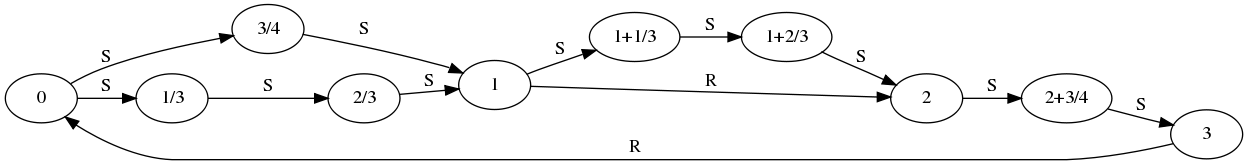
\includegraphics[width=12cm]{rythm_markov/images/grafo_con_etiquetas.png}
\label{fig:grafo_con_etiquetas}
\end{center}
\end{figure}

Esta \'ultima aproximaci\'on asume que el silencio es un elemento que est\'a a la misma altura que el sonido, cosa que no es asi. 
De esta forma, el modelo no tendr\'a etiquetas en las aristas y no diferenciar\'a entre silencio y sonido.

\begin{figure}[h]
\begin{center}
\includegraphics[width=12cm]{rythm_markov/images/grafo_con_silencios_sin_etiquetas.png}
\label{fig:grafo_con_etiquetas}
\end{center}
\end{figure}

Para generar un comp\'as sencillamente se recorre la cadena de markov, hasta que el estado actual sea menor que el proximo estado determinado por la cadena

\subsection{Formalmente}
Dado $C \in \Nat$ (posiblemente $C=m$), se define a la cadena de markov como una tripla $<V, E, P>$ donde $V$ es el conjunto de estados, $E$ el conjunto de aristas y $P$ una distribuci\'on de probabilidad sobre las transiciones.
Dada una partitura $P = \Score$ 
\begin{itemize}
    \item $V = \{ go_i\bmod C, \forall i, i \le n+k \}$
    \item $E = \{ (go_i \bmod C, go_{i+1} \bmod C), \forall i, i < n+k \}$
    \item Sean $n_1, n_2 \in V$, entonces $P(n_2 | n_1) = \frac{|n_1 \rightarrow n_2|}{|n_1|}$ donde
        \begin{flalign}
        |n_1 \rightarrow n_2| &= |\{(go_i, go_{i+1}) \text{ tal que } go_i \equiv n_1 \pmod C \land go_{i+1} \equiv n_2 \pmod C  \}| \\
        |n_1|                 &= |\{go_i \text{ tal que } o_i\equiv n_1\pmod C \}|
        \end{flalign}
\end{itemize}    

\end{document}
